% -*- mode: LaTex; outline-regexp: "\\\\section\\|\\\\subsection";fill-column: 80; -*-
\documentclass[12pt]{article}
\usepackage[longnamesfirst]{natbib}
\usepackage[usenames]{color}
\usepackage{graphicx}  % Macintosh pdf files for figures
\usepackage{amssymb}   % Real number symbol {\Bbb R}
\input{../../standard}

% --- margins
\usepackage{../../sty/simplemargins}
\setleftmargin{1in}   % 1 inch is NSF legal minimum
\setrightmargin{1in}  % 1 inch is NSF legal minimum
\settopmargin{1in}    % 1 inch is NSF legal minimum
\setbottommargin{1in} % 1 inch is NSF legal minimum

% --- Paragraph split, indents
\setlength{\parskip}{0.00in}
\setlength{\parindent}{0in}

% --- Line spacing
\renewcommand{\baselinestretch}{1.3}

% --- Margins
\setlength{\topmargin}{-0.5in}
\setlength{\oddsidemargin}{-0.1in}
\setlength{\textheight}{9.0in}
\setlength{\textwidth}{6.5in}

% --- page numbers
\pagestyle{empty}  % so no page numbers

% --- Hypthenation
\sloppy  % fewer hyphenated
\hyphenation{stan-dard}
\hyphenation{among}

% --- Customized commands, abbreviations
\newcommand{\TIT}{{\it  {\tiny Optimal Alpha Investing (DRAFT) (\today)}}}

% --- Header
\pagestyle{myheadings}
\markright{\TIT}

% --- Title

\title{ Optimal Streaming Feature Selection  }
\author{
        Robert A. Stine\thanks{Research supported by NSF grant DMS-1106743 }  \\
        Department of Statistics            \\
        The Wharton School of the University of Pennsylvania \\
        Philadelphia, PA 19104-6340                          \\
        www-stat.wharton.upenn.edu/$\sim$stine 
}

\date{\today}

%%%%%%%%%%%%%%%%%%%%%%%%%%%%%%%%%%%%%%%%%%%%%%%%%%%%%%%%%%%%%%%%%%%%%%%%%%%

\begin{document}
\maketitle 
%------------------------------------------------------------------------

\abstract{ 

 Streaming feature selection identifies variables to add to a model by testing a
 sequence of proposed variables. Rather than specify a set of explanatory
 variables as in the typical stepwise regression, streaming selection allows the
 search for predictors to adapt to the success of prior choices.  The choice of
 the next variable can depend on results of prior tests.  To avoid over-fitting,
 alpha-investing controls the expected false discovery rate (mFDR) of these
 sequential tests. Alpha investing rules, however, provide the modeler with
 considerable flexibility in both the selection of features to test as well as
 the alpha-level committed to each test. Our work here identifies optimal
 strategies for alpha investing that perform within a tolerance of the best
 possible. The modeler is then free to focus on strategies for choosing the next
 explanatory variable rather than setting the level of the next test. We show
 that a spending rule based on a universal prior is competitive with an oracle
 that knows the strategy of the modeler and sets the signal of the tested
 hypothesis. We also consider the risk-ratio of the selected model vis-a-vis
 that of the oracle model.

}

%------------------------------------------------------------------------
\vspace{0.05in}

\noindent
{\it Key Phrases: } 

\begin{itemize}
  \item note that we find the convex hull of the feasible set of solutions
  \item we start the universal at 1
  \item universal is above, below, then ultimately above others
  \item try things with uniform since it saves the most among monotone
  \item bulge solved by rotating gamma?
  \item Why the up down for the fits with gamma 0.025?
\end{itemize}

\clearpage


% ----------------------------------------------------------------------
\section{Testing Game}
% ----------------------------------------------------------------------

 The choice of an optimal spending plan is difficult to formulate in total
 generality, but a special case related to information theory suggests a general
 plan.  We call this case the 'testing game' to remind us all that it is
 contrived.  In the game, a player (the statistician) is confronted by a
 sequence of null hypotheses $H_1$, $H_2, \; \ldots$ chosen by Nature.  The
 objective of the player is to detect a false null hypothesis positioned by
 Nature within this sequence.  The false null is $H_K$, where $0 < K$ is a
 random variable with monotone decreasing probabilities, $P(K=k)=p_k, \,
 k=1,2,\ldots$.  The player begins the game with alpha-wealth $0 \le W$, and
 {\em at the start} of the game and without knowing the distribution $p$, the
 player must announce a plan for how this wealth will be invested in testing the
 sequence of hypotheses.  That is, the player commits to invest $q_1W$ to the
 test of $H_1$, $q_2W$ to the test of $H_2$ and so forth, with $\sum q_j = 1$
 with $0 \le q_j$ ($q$ is a discrete probablity distribution). The player wins
 the amount $g(q_K W)$ where $g$ is a monotone non-decreasing function.  The
 more the player commits to testing the false null, the more the player wins.
  The question is then ``How should the player allocate the alpha-wealth $W$?''


 If the player knows Nature's probability distribution $p$ and the payoff
 function $g = \log$, then the optimal allocation is an immediate property of
 the divergence (or Jensen's inequality).  The divergence (or relative entropy)
 between two discrete probability distributions is
 \begin{equation}
   \divg{p}{q} = \ev_p \log \frac{p}{q} 
               = \sum_j \log\left(\frac{p(j)}{q(j)}\right) p(j) \ge 0 \;.
 \label{eq:divg}
 \end{equation}
 In this special version of the Testing Game, the expected amount won is $\ev
 g(q_KW) = \ev \log q_K W \le \ev \log p_K W$ because the divergence is
 non-negative.  The best strategy is to allocate the alpha-wealth according to
 the probabilities used by nature to pick the location of the false null.  In
 this contrived setting, the Testing Game is equivalent to finding the binary
 code for $K$ with the shortest expected length.  The solution is well known to
 be the binary code with length determined by the probability distribution of
 $K$.  \ras{Can there be any further generality, even here, such as to other
 functions than log? I thought so, but log is special in that $\log x - \log y =
 \log(x/y)$ allows one to play the Jensen game in showing the divergence is
 positive.}


 Information theory also supplies a solution to the more general problem of
 allocating $W$ when $p$ is unknown.  Assume now that Nature picks the
 distribution $p$ after the player announces the strategy $q$, with the goal of
 minimizing the expected winnings of the player.  The player now needs a
 strategy $q$ which solves the minimax problem
 \begin{equation}
   \max_q \min_p \ev g(q_K)   
 \label{eq:qopt}
 \end{equation}
 Provided we limit nature to monotone decreasing distributions for which
 $p_{k+1} \le p_k$ and keep $g = \log$, the optimal strategty of the player is
 to use the universal distribution of \citet{elias75, rissanen83}.  A simple
 version of the universal distribution is given by the distribution
 \begin{equation}
   u_j = \frac{c_u}{j + \log (1+j)} \;, \quad j = 1,\,2\, \ldots,
 \label{eq:univ}
 \end{equation}
 where the constant $c_j \approx 3.388$ normalizes the sum so that $\sum u_j = 1$.


 The Testing Game motivates the use of the universal spending rule $u$, but the
 risk of the estimator implied by this approach are unknown.  Suppose that the
 universal distribution is used to define an alpha-investing rule.  Then, since
 tests produced by following an alpha-investing rule control mFDR, we know that
 the sequence of tests defined by the universal distribution control false
 positives in this sense as well.  Optimality in the Testing Game, however, does
 not imply optimality in the false discovery rate.  We further do not know the
 risk associated with this procedure.  To describe the risk, assume that the
 hypotheses being tested are of the form $H_j: \mu_j = 0$ with available test
 statistics $\ol{y}_1$, $\ol{y}_2, \,\ldots$.  The tests then define estimators
 (testimators)
 \begin{equation}
    \hat\mu_j = \left\{ 
       \begin{array}{cc}
           0         & \mbox { if $H_j$ is not rejected, }    \cr
           \ol{y}_j  & \mbox { otherwise. } 
       \end{array}  \right.
 \label{eq:muhat}
 \end{equation}
 Such testimators are equivalent to hard thresholding with the threshold set
 adaptively by the allocated alpha-level.

 
 Our objective here is to understand the risk of these estimators.


\clearpage



% ----------------------------------------------------------------------
\section{Introduction}
% ----------------------------------------------------------------------


 Emphasize that we have a computational approach that determines an attainable
 upper bound on the risk rather than a mathematical procedure that gives an
 inequality that obtains asymptotically with error terms (stat) or with some
 high probability (mach learning style).  We obtain nonasymptotic results in
 moderate size problems, with the scope of the results limited only by
 computing.


 Note that there are not results (?) that connect FDR to the risk of the
 associated estimators.  We might be able to do that, though not clear to me how
 we can keep track of the growing/necessary state.

 
 Our results are in a different style in that not just the nearly black sparse
 setting, but rather more general.

 
 Convexity. A simple randomization argument shows that any linear combination of
 the mean points that we found is attainable.  That's not the same, however, as
 showing that the actual set is convex.  Each calculation we do (for some gamma
 or direction angle) finds the maximum value of the function in that direction.
  Hence, you cannot get further out in that direction. That removes half of the
 space; a collection of these leaves a convex interior.  That convex interior
 holds the collection of solutions.  The smaller the angle between direction
 vectors, the closer we approximate the feasible set.  Rather than get the
 intersection of {\em all} half-spaces that hold the feasible region, we git a
 finite number of them.




 Streaming feature selection is a sequential method for identifying predictive
 features for a model.  Rather than choose the best feature from a fixed,
 predetermined collection, streaming feature selection evaluates candidate
 predictors one-at-a-time, following an order specified by an exogenous source.
  Unlike stepwise regression, streaming selection evaluates each predictor in
 the context of the current model, without knowledge of others that might
 follow.  Sequential feature selection allows the evaluation of initial features
 to generate others, allowing the model to consider infinite sequences of
 explanatory variables. Alpha-investing provides control of over-fitting in this
 context without the sacrifice of data to cross-validation.


 As an example for comparison, consider the familiar setting in which one
 observes $p$ vectors of features $x_j \in \Rn$ to consider using as explanatory
 variables in a model to predict a response $y \in \Rn$.  The classical version
 of this problem is the choice of features for the homoscedastic linear
 regression model
 \begin{equation}
   y_i = \beta_0 + \beta_1 x_{i1} + \cdots + \beta_p x_{ip} + \ep_i, 
     \qquad \ev \ep_i = 0, \Var(\ep_i)=\sigma^2,
 \label{eq:homo}
 \end{equation}
 in which many $\beta_j \approx 0$.  Forward stepwise regression is perhaps the
 earliest algorithmic approach to identifying the variables with statistically
 interesting, non-zero coefficients.  Stepwise regression begins by selecting
 the variable, say $x_{(1)}$, that has the largest correlation with $y$,
 $x_{(1)} = \arg \max_{x_j} \corr(x_j,y)$.  The algorithm continues adding
 variables $x_{(2)},\, x_{(3)}, \ldots$ until some stopping criterion is
 reached, such as AIC or BIC.  In the somewhat utopian case in which the
 observed vectors $x_j$ are orthonormal ($x_j'x_k = I_{\{j=k\}}$) and one has an
 independent estimate $s^2$ of $\sigma^2$, one can use Bonferroni (hard
 thresholding).  The least squares estimators are $b_j = x_j'y.$ This criterion
 picks those variables for which the usual t-statistic $t_j = b_j/s$ exceeds the
 threshold $\tau \approx \sqrt{2 \log p}$.  Further improvements related
 to FDR reduce the threshold adaptively.

 
 Streaming feature selection operates differently.  An exogenous source
 determines the first feature to examine.  Rather than find the feature that
 maximizes the correlation with $y$ among all $p$ possible variables, streaming
 selection begins with the first variable that a researcher selects.  For
 example, a scientist might order the genes to consider when modeling their
 impact on disease in a micro-array experiment, or an economist might have a
 particular pet variable or theory that explains unemployment.  In any case, we
 assume that the indexing of the explanatory variables reflects this precedence.
  A streaming selection algorithm then tests this first variable $x_1$ for
 statistical significance using some variation on the usual $t$-statistic, say
 $t_1$.  For this paper, we assume that this statistic is computed
 conservatively in the manner of \citet{fosterstine04:bank}.  If the initial
 $t$-statistic exceeds a threshold, $|t_1| > \tau_1$, the algorithm adds $x_1$
 to the regression model.  Otherwise, the model is left empty.  Whether $x_1$
 joins the model or not, the algorithm continues on to examine the second
 variable, with the choice of $x_2$ possibly influenced by the outcome of the
 initial test.  The geneticist, for instance, might alter the choice of the gene
 represented by $x_2$ depending on whether $x_1$ was selected into the model.
  Alternatively, a scientist might decide to use the variable $x_2 = x_1^2$ or
 some other transformation of $x_1$ depending on the outcome of the first test.
  Although one begins with a predefined set of $p$ features, this ability to
 combine and transform variables dynamically expands the scope of the search.
  If the $t$-statistic exceeds the next threshold, $|t_2| > \tau_2$, $x_2$ joins
 the model.  The search then moves on to consider the next variable.  Our
 results here consider methods for setting the sequence of thresholds $\tau_1,
 \tau_2, \ldots$.


 This illustration highlights two characteristics that separate streaming
 feature selection from stepwise selection.  The first characteristic collects
 the advantages of streaming selection, and the second implies the need for a
 different means to control the selection of variables.
 \begin{description}
  \item[One feature is considered at each step of streaming feature selection]
 This step leads to an evident speed advantage over stepwise selection and means
 that one evaluates the statistical significance of $x_j$ quite differently from
 the method applied to $x_{(j)}$.  The stepwise choice $x_{(j)}$ must exceed a
 threshold for significance derived from the maximum of a collection of test
 statistics, whereas the test of $x_j$ does not. Consequently the streaming
 threshold is possibly much smaller ($\tau_1 < \tau_{(1)}$), offering gains in
 power --- provided the exogenous ordering is reasonable.
  \item[The scope of the streaming search is not initially known] In particular,
 the number of possible features considered in the search is allowed to change
 as the search proceeds.  The initial collection is allowed to expand to include
 powers $x_j^2$, interactions $x_j\,x_k$, functional transformations $g(x_j)$,
 and so forth.
 \end{description}
 The sequential, unbounded nature of the search requires an adaptive means of
 setting the sequence of thresholds $\tau_, \tau_2, \ldots$.  Because one does
 not know the size of the search space or the full collection of features to be
 considered, methods such as AIC or Bonferroni are not suited to controlling the
 search in streaming feature selection.


% ---------------------------------------------------------------------------
\section{Alpha Investing}
% ---------------------------------------------------------------------------

 Alpha investing \citep{fosterstine08} is a method for testing a possibly
 infinite sequence of hypotheses, designed with this application to model
 selection in mind.  Alpha investing begins with an initial allocation $W_1$ of
 alpha wealth; alpha wealth is the current total alpha level that can be spent
 to test subsequent hypotheses.  Label a sequence of null hypotheses $H_1, H_2,
 \ldots$, such as the sequence $H_j: \beta_j=0$ in regression.  An alpha
 investing rule can test $H_1$ at any level up to the total available alpha
 wealth, $0 \le \alpha_1 \le W_1$.  The level $\al_1$ is 'spent' and cannot be
 used for subsequent tests.  Let $p_1$ denote the p-value of the test of $H_1$.
  If $p_1 \le \alpha_1$, the initial test rejects $H_1$.  In this case, the
 alpha investing rule earns an additional contribution $\omega >
 0$ \marginpar{$\omega$} to its alpha wealth; otherwise, the alpha wealth
 available for subsequent tests falls to $W_2 = W_1 - \alpha_1$.  We typically
 set $\omega = 0.05$ in applications.  In general, the alpha wealth available for
 the test of $H_{j+1}$ is \marginpar{$W_j$}
 \begin{equation}
    W_{j+1} = W_j - \alpha_j + \omega \, I_{\{p_j < \al_j\}}
 \label{eq:Wj}
 \end{equation}
 Alpha investing resembles alpha spending used in clinical trials, with the key
 distinction that rejecting a hypothesis earns an additional allocation $\omega$
 of alpha wealth for subsequent testing.  An alpha spending rule, such as the
 Bonferroni rule, controls the family wide error rate (FWER).  FWER is the
 probability of falsely rejecting any null hypothesis.  An important special
 case is control of FWER under the so-called complete null hypothesis for which
 $H_j$ holds for all tests.  We refer to controlling FWER under the complete
 null hypothesis as controlling FWER in the weak sense.  


 With the possible injection of additional alpha wealth, alpha investing weakly
 controls FWER and a version of the false discovery rate (FDR).  Let $R(j)$
 count the number of hypothesis rejected in the first $j$ tests, and let $V(j)
 \le R(j)$ denote the number of false rejections through the first $j$ tests.
  Then we can define the criterion
 \begin{equation}
    \mbox{mFDR}(j) = \frac{\ev V(j)}{1+\ev R(j)} \;.
 \label{eq:mFDR}
 \end{equation}
 FDR uses the expected value of the ratio whereas mFDR uses the ratio of
 expected values.  \citet{fosterstine08} show that alpha investing controls
 $\mbox{mFDR}(j) \le \omega$, and this result implies weak control of the FWER.
  The index $j$ is allowed to be an arbitrary stopping time, such as the
 occurrence of the $k$th rejection.

 
 Although the ordering of the variables to consider for selection in a model is
 key to the success of streaming feature selection, we show in this paper that
 the investigator need not be so concerned about how to set the sequence of
 levels $\alpha_j$.  Basically, we demonstrate alpha investing rules that
 perform as well as competitors that know the underlying parameters.  The use of
 such a rule allows the investigator to focus on the search strategy rather than
 nuances of the choice of $\alpha_j$.  For our analysis, we consider alpha
 investing rules that are defined by a monotone discrete distribution on
 non-negative integers.  Let ${\cal F} = \{f:\{0,1,\ldots\} \mapsto \R^{+}, \, f(j)
 \ge f(j+1),\, \sum_j f(j) = 1\}$ denote the collection of monotone,
 non-increasing probability distributions on the non-negative integers.  Each $f
 \in {\cal F}$ defines an alpha investing rule that `resets' after rejecting a
 null hypothesis.  Given the wealth after rejecting some hypothesis $H_{k-1}$ is
 $W_{k}$, then the levels for testing subsequent hypotheses $H_{k+j}, \,
 j=0,1,\ldots,$ are $\al_{k+j} = W_k \; f(j)$, until the next rejection.
  Monotonocity implies that the alpha investing rule spends more heavily after
 rejecting a hypothesis than otherwise; such rules are suitable in applications
 in which significant factors cluster, as if non-zero $\mu_j$ occur in bundles.
  \citet{fosterstine08} offer further motivation for this approach.

 
 We focus on two members of this class of alpha investing rules: those
 identified by a geometric distribution and by a universal distribution.
  Geometric alpha investing rules spend a fixed fraction $\psi$ of the current
 wealth on each round.  Let $g_\psi(j) = \psi(1-\psi)^{j},\, j=0,1,\ldots,$
 denote the geometric distribution with parameter $0 < \psi <
 1$.  \marginpar{$g_\psi, \psi$} For example, the geometric rule with $\psi =
 0.25$ invests one-fourth of the current alpha wealth in the test of $H_j$,
 $\alpha_j = W_j/4$.  In general, given wealth $W_{k}$ after rejecting
 $H_{k-1}$, say, the amount invested in testing $H_{k+j}$ is $\alpha_{k+j} = W_k
 \, g_\psi(j)$.  Large values for $\psi$ rapidly spend down the alpha wealth
 available after a rejected hypothesis.  Geometric investing is natural and
 related to entropic approximations to distributions.  That is, given a fixed
 set of initial probabilities, assigning a geometric tail to the distribution
 minimizes the relative entropy of the approximation (cite).


 The second alpha investing rule uses a version the universal prior for integers
 defined by \citet{rissanen83}.  The universal prior arises in the context of
 encoding a sequence of positive integers using a prefix code.  A geometric rule
 spends a constant fraction of the wealth on each test.  The universal rule
 instead invests a diminishing proportion of the available alpha wealth.  Of the
 wealth $W_k$ available after a rejecting $H_{k-1}$, say, the universal rule
 invests $\al_{k+j} = W_k\,u(j)$ with
 \begin{equation}
   u_\delta(j) = \frac{c}{ (j+\delta) (\log (1+j+\delta))^2}, \qquad 
                 j =  0,\,1,\,\ldots, \quad 1 \le \delta.
 \label{eq:univ}
 \end{equation}
 in the tests of $H_{k+j}$ until the next rejection. ($c_\delta$ is a
 normalizing constant so that the discrete probabilities $u_\delta(j)$ add to 1;
 for example, $c_{1} \approx 3.388$ and $c_{20} \approx 0.3346$.)  The constant
 $\delta$ \marginpar{$\delta$} serves as an offset that slows the initial
 spending rate; our examples fix $\delta=20$ and we abbreviate $u_{20}(j) =
 u(j)$. (For instance, $u_1(0) \approx 0.614$ so that the rule spends about 60\%
 of the available wealth on the first test.)  More elaborate forms of the
 universal distribution make use of the so-called log-star function, defined as
 $\log^* x = \log x + \log \log x + \cdots$, where the sum accumulates only
 positive terms.  For example, $\log^{*} 8 = \log 8 + \log \log 8$.  The version
 \eqn{eq:univ} simply uses the first two summands of the $\log^{*}$ function.
 


%--------------------------------------------------------------------------
\section{Optimal Alpha Investing}
%--------------------------------------------------------------------------
 
 To evaluate an alpha investing rule, we consider its performance in the
 following context.  Consider testing a sequence of $T$ one-sided null
 hypotheses $H_j: \mu_j \le 0, \, j=1,\,2,\, \ldots, \mu_T$ versus the alternatives
 $H_{j,a}: \mu_j > 0$.  \marginpar{$\mu_{1:T}$} Denote the collection of mean
 parameters $\mu_{1:T} = \{\mu_1, \mu_2, \ldots, \mu_T\}$.  The test statistics
 are $Z_j \sim N(\mu_j,1)$.  The $Z_j$ are independent and observed one at a
 time; the test of $H_k$ is made in the knowledge of prior $Z_j$ for $j<k$, but
 future $Z_j, j > k$ are unknown.  The number of tests $T$ is fixed and known at
 the start of testing.  For the purpose of calculating risks, a sequence of
 tests defines a sequence of `testimators' by setting $\hat\mu_j = Z_j$ if
 $p_j<\al_j$ and zero otherwise.
 

 Within this context, how does the choice of an investing rule influence the
 performance of alpha investing?  Let $U$ denote a figure of merit, or utility,
 provided by using an alpha investing rule.  For example, the utility might be
 the expected number of hypothesis $H_j:\mu_j=0$ rejected by the alpha investing
 rule defined by the distribution $f \in {\cal F}$:
 \begin{eqnarray}
    U_r(\mu_{1:T},\,f) 
      &=& \ev_{\mu_{1:T}} \sum_{j=1}^T r_{\mu_j}(\alpha_j) \label{eq:Ur} \\
      &=& r_{\mu_1}(\al_1) \left( 1 + r_{\mu_2}(W_1-\al_1+\omega) + \cdots \right)\cr
      & &  + (1-r_{\mu_1}(\al_1))\left( r_{\mu_2}(W_1-\al_1) + \cdots \right) \;,
 \label{eq:Ure}
 \end{eqnarray}
 where $r_\mu(\al) = \Phi(\mu - z_\alpha)$ is the probability of rejecting,
 $z_\al = \Phi^{-1}(1-\al)$ is the normal quantile, and $\Phi$ is the cumulative
 standard normal distribution.  In \eqn{eq:Ur}, $\al_j$ denotes the amount
 invested in the test of $H_j$ by following the investing rule defined by the
 distribution $f$; this notation suppresses the detail of how prior rejections
 influence this random variable as suggested by \eqn{eq:Ure} that shows how
 $\al_2$ depends on the prior outcome.  Alternatively, we also measure the
 utility in the sense of accumulated (negative) risk.  If $Z \sim N(\mu,1)$,
 then the risk of the testimator $\hat\mu = Z \,I_{\{Z < z_\al\}}$ is
 \begin{equation}
   R_{\mu}(\al) = (1-r_\mu(\al))\mu^2 + (z_\al-\mu)\phi(z_\al-\mu) + \Phi(\mu-z_\al)
 \label{eq:Rmu}
 \end{equation}
 The associated cumulative utility is then
 \begin{equation}
    U_R(\mu_{1:T},\,f) = \ev_{\mu_{1:T}} \sum_{j=1}^T R_{\mu_j}(\alpha_j) 
 \label{eq:UR}
 \end{equation}
 

 To compare two alpha investing rules defined by $f,\,g \in {\cal F}$, define
 the {\em performance envelope} of $(f,\,g)$ to be the region
 \begin{equation}
    \mbox{PE}(f,g;\rho) = \{(x,\,y) \in \R^2: \exists \; \mu_{1:T} \in \RT \; s.t. \; 
                     x = U_\rho(\mu_{1:T},f),\,  y=U_\rho(\mu_{1:T},g))\} \;.
 \label{eq:PE}
 \end{equation}
 The point $(x,\,y)$ lies in the performance envelope if there exists a sequence
 of means for which these coordinates identify the utilities obtained by the two
 alpha investing rules.  As an example, Figure \ref{fi:pe} shows PE$(g_{0.11},u;\;
 r)$, the rejection performance envelope of alpha investing with a geometric
 distribution having $\psi = 0.11$ versus the universal distribution $u$ defined
 in \eqn{eq:univ}.  Points within the performance envelope of $(g_{0.11},u)$ that lie
 below the diagonal indicate parameters $\mu_{1:T}$ for which $g_{0.11}$ produces
 higher utility than $u$; those above the diagonal (the larger portion of Figure
 \ref{fi:pe}) indicate $u$ dominates $g_{0.11}$. In this example, the universal
 distribution dominates the geometric almost everywhere.  The advantage is
 particularly stark near the origin; in this `nearly black' situation, few
 hypotheses are rejected and the universal rule produces far better performance.


 \begin{figure}
 \caption{ \label{fi:pe} Performance envelope PE$(g_{0.11},u;\;r)$ shows the
 expected number of rejected hypotheses obtained by the geometric alpha
 investing rule $g_{0.11}$ versus the universal investing rule ($T=250$)}
 \centerline{ 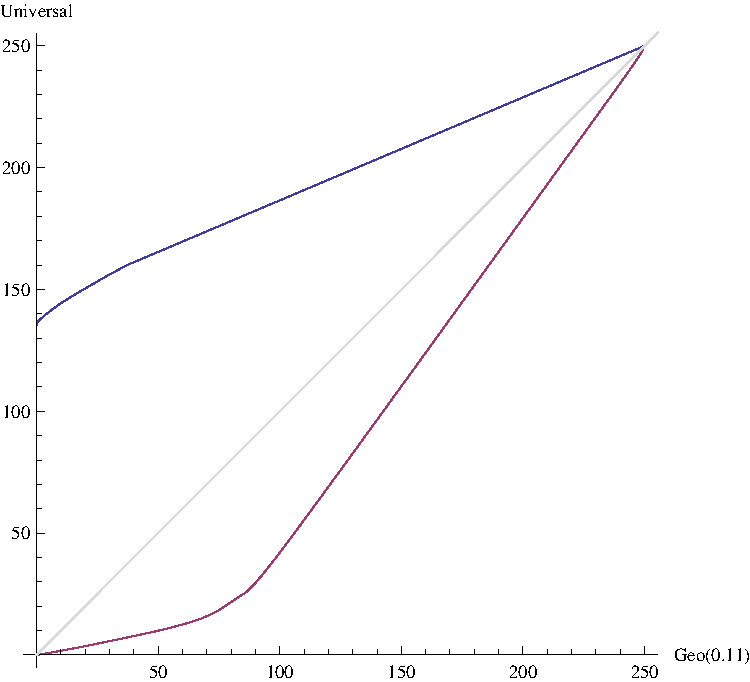
\includegraphics[width=4in]{envelope} }
 \end{figure}



%--------------------------------------------------------------------------
\section{Finding the Performance Envelope}
%--------------------------------------------------------------------------

 We identify the boundary of the performance envelope by solving a collection of
 one-dimensional optimizations.  Figure \ref{fi:tangent} illustrates the method
 used to identify a boundary point of PE$(f,g; r)$ that lies above the diagonal.
  Pick some value $\gamma > 0$ \marginpar{$\gamma$}; $\gamma = 1$ in the figure.
  The intercept $C^\gamma$ of the tangent line identifies the boundary value of
 the performance envelope at the point of tangency:
 \begin{equation}
     C^\gamma = \max_{\mu \in \RT} U_r(\mu,g) - \gamma \, U_r(\mu,f) 
 \label{eq:opt}
 \end{equation}
 The solution is obtained recursively as in a Bellman equation.  To express the
 recursion, expand the notation and let $C^\gamma = C_1^\gamma(A_1,0;B_1,0)$
 where $A_1=B_1=W_1$ denote the initial alpha wealths associated with the alpha
 investing rules defined by $f$ and $g$. The zeros indicate that no tests have
 occurred since the last rejection so that $f(0)$ and $g(0)$ determine the amount
 to invest in the test of $H_1$.


 \begin{figure}
 \caption{ \label{fi:tangent} The intercept of the tangent line with slope
 $\gamma = 1$ identifies a point on the boundary of the performance envelope. }
 \centerline{ 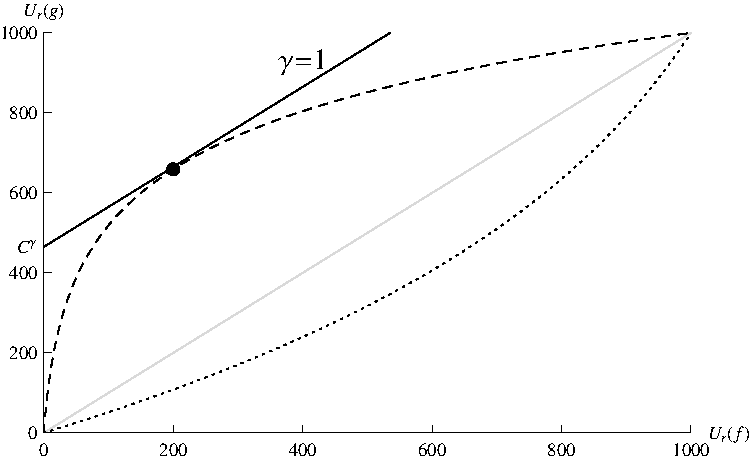
\includegraphics[width=4in]{tangent} }
 \end{figure}

 
 Now consider the general case of the test of $H_j$.  Assume that the alpha
 wealth available to the two investing rules is $A_j$ and $B_j$, respectively,
 at this stage, and that it has been $\ell \le j$ tests since the last rejection
 by the first rule and $m \le j$ tests since the last rejection by the second.
  Assume also for ease of presentation that the level $\al_j = A_j f(\ell)$
 invested in the test of $H_j$ by the first investing rule is less than the
 level $\beta_j = B_j g(m)$ invested by the second ($\al_j < \beta_j$). It
 follows that, when utility is measured by the number of rejections, that we
only need a one-dimensional optimization at each test,
 \begin{eqnarray}
   C^\gamma_j(A_j,\ell;B_j,m) 
    &=& \max_{\mu \in \R } \left[ r^{}_{\mu}(\al_j) - \gamma \, r_{\mu}(\beta_j)\right. \cr
    && \;+ \quad r_{\mu}(\al_j) \qquad \quad
              C^\gamma_{j+1}(A_j+\omega-\alpha_j,0;\,B_j+\omega-\beta_j,0)  \cr
    && \;+ (r_\mu(\beta_j)-r_\mu(\al_j)) \; 
              C_{j+1}^\gamma(A_j-\alpha_j,\ell+1;\,B_j+\omega-\beta_j,0) \cr
    && \;+ \left.  (1-r_\mu(\beta_j)) \; 
              C_{j+1}^\gamma(A_j-\alpha_j,\ell+1;\,B_j-\beta_j,m+1) \right] \;,
 \label{eq:util}
 \end{eqnarray}
 with the boundary condition $C_{T+1}^\gamma = 0$.  The successive lines
 identify the expected differential in the number of rejections produced by the
 test of $H_j$, and following summands denote the subsequent expected values if
 both reject, if only the rule with the larger alpha level rejects, and if
 neither rejects.  


 Practical solution of the recursion for $C_1^\gamma$ requires a discrete
 approximation.  Notice in \eqn{eq:util} that the state of the recursion depends
 on the wealths of the two investing rules. Feasible calculation requires that
 we restrict the possible wealths to a discrete grid.  If the wealths are
 allowed to vary over any $W \ge 0$, then solving this recursion for any sizable
 $T$ is intractable.  Our approach discretizes the wealth functions so that the
 optimization occurs over a grid for each test $j$ rather than the positive
 quadrant of $\R^2$.  For each investing rule, we initialize a grid of $T+M+1$
 wealth values $w_j$, indexed from $j=M, M-1, \ldots, 1, 0, -1, \ldots, -T+1,
 -T$.  This grid holds the state of the wealth at each test, and the differences
 in adjacent wealths determine the amounts used to test the next hypothesis.
  For the rule defined by the distribution $f \in {\cal F}$, we set $w_0 = W_1$,
 $w_{-1} = w_0(1-f(0))$, $w_{-2} = w_{-1}(1-f(1)), \ldots$.  If the investing
 rule does not reject any hypotheses, these wealths are exact.  If the rule does
 reject, we accumulate the utility as though performing a randomized test that
 tosses a biased coin to decide which of the nearby wealths to spend.  Suppose
 that the alpha wealth when rejecting is $x = w_j + \omega$.  It is unlikely
 that $x$ lies at one of the grid of wealth values, so assume that $x = c \, w_k
 + (1-c) w_{k+1}$ for some $0 < c < 1$.  In this case, we treat the next test as
 a randomized test.  The test earns the expected utility from wealth $w_k$ with
 probability $(1-c)$ and from wealth $w_{k+1}$ with probability $c$. Basically,
 this approximation adds a second expectation to the sum in \eqn{eq:util}. We
 set $w_j$ for $j > 0$ somewhat arbitrarily in a manner that prevents the
 accumulation of excess wealth.  In our examples, $M=5$ with $w_i = W_1 + i
 \,\omega/3$, $i=1,2,3$, and $w_i = w_{i-1} + \omega$ for $i=4,\,5$.  Should the
 wealth reach $w_4$, then the bid for the next test is $\omega$, the amount
 earned by a rejection.  Hence, the testing does not increment the wealth beyond
 this boundary.
 

 We obtain a performance envelope by varying the competitive factor $\gamma$.
  To find the boundary points below the diagonal, we reverse the roles of the
 alpha investing rules and repeat the optimization.  As the optimization
 proceeds, we accumulate the component utilities that identify the boundary
 point.



%--------------------------------------------------------------------------
\section{More results, mean choices}
%--------------------------------------------------------------------------


%--------------------------------------------------------------------------
\section{Discussion}
%--------------------------------------------------------------------------

Alpha investing can mimic regular testing procedure by revisiting the test of
prior hypotheses. 

One might also use accumulated alpha wealth as a measure of the performance, and
 this provides a more useful metric of performance, particularly when competing
 against the oracle.  If maximizing alpha wealth, then the oracle loses the
 amount bid and chooses $\mu_j$ to maximize $r_{\mu_j}(\al)-\al$ rather than
 $r_{\mu_j}(\al)$ alone.  This perspective would not only capture aspects of
 rejecting hypotheses, it also anticipates having resources to test future
 hypotheses.  Such consideration is appropriate, however, only in the context of
 testing a larger collection of hypotheses than considered here.

 \ras{ Things left to do:
 \begin{enumerate}
 \item Graphs of envelope that suggest that alpha wealth is a decent proxy for
 risk, at least better than something like FDR, number rejects - constant times
 number false rejects.
 \item What does the steady state look like.  If take the envelope for 250 and
 double to get for 500, is that close to correct for the risk?
 \item Comment on the value of saving if hope to compete with a universal
 bidder.
\end{enumerate}
}


%--------------------------------------------------------------------------
\section*{Acknowledgement}
%--------------------------------------------------------------------------

The authors thank ...


%--------------------------------------------------------------------------
% References
%--------------------------------------------------------------------------

\bibliography{../../../../references/stat}
\bibliographystyle{../../bst/asa}

\end{document} %==========================================================
